\documentclass[a4paper, 11pt]{article}
\usepackage{graphicx}
\title{Using DIALS}
\author{Graeme Winter, Diamond Light Source}

\begin{document}

\maketitle

\section{Caveat Lector}

These are my notes on how to run elements of the DIALS processing suite. I make no promises that anything described in here will work, or will give sensible results, or will in fact do anything. You have been warned.

\section{Introduction}

DIALS processing may be performed by either running the individual tools (spot finding, indexing, refinement, integration, exporting to MTZ) or you can run the whole lot through \verb|dials.process|, which just chains them together (and incidentally does all of the processing in P1.)

\section{dials.process}

In the simplest case, \verb|dials.process /here/are/all/images*.cbf| will do  sensible processing, with a static model of the experiment and sample, and will output a reflection file \verb|integrated.mtz| containing the intensity measurements assuming everything works correctly. Some sensible options to use are:

\begin{itemize}
\item{\verb|scan_varying=true| - allow the crystal orientation and unit cell constants to vary during the scan}
\item{\verb|--nproc=1| - only use one processor (necessary currently for data in NeXus files}
\item{\verb|intensity.algorithm=sum2d| - use 2D summation integtration rather than the default 3D summation, other algorithms are being added}
\item{\verb|shoebox.n_blocks=N| - for some N, split the data set into N blocks for integration, so as not to overload the computer} [NKS FIXME:  what is a block?]
\item{\verb|-i| - pass the images to process through the standard input e.g. from \verb|find . -name '*.cbf'| to avoid issues with limited command-line lengths}
\end{itemize}

\noindent
I have used all of these options and they appear to do sensible things. Important to make sure that what is passed in is exactly one sweep.

\section{Results}

At the start you will see:

{\small
\begin{verbatim}
********************************************************************************

                       mmmm   mmmmm    mm   m       mmmm            
                       #   "m   #      ##   #      #"   "           
                      m#mm  #   #     #  #  #      "#mmm            
                       #    #   #     #mm#  #          "#           
                       #mmm"  mm#mm  #    # #mmmmm "mmm#"           

Launching dials.process

The following tasks will be performed:
 1) Strong spots will be found (dials.find_spots)
 2) The strong spots will be indexed (dials.index)
 3) The model will be further refined (dials.refine)
 4) The reflections will be integrated (dials.integrate)
 5) The data will be exported as MTZ (dials.export_mtz)

Please be patient, this may take a few minutes

********************************************************************************

Command-line: scan_varying=true /Users/graeme/data/i04-BAG-training/th_8_2_0001

********************************************************************************
\end{verbatim}
}

\noindent
and depending on the size of your data set you may be looking at this
for a while. The first thing to happen is the peak finding, which
happens for every image in the set (this will probably be changed in
the future.)

{\small
\begin{verbatim}
********************************************************************************
Finding Strong Spots
********************************************************************************
Configuring spot finder from input parameters
--------------------------------------------------------------------------------
Finding strong spots in imageset 0
--------------------------------------------------------------------------------

Finding spots in image 0 to 540...
Extracted strong pixels from images......................................210.62s
Merged 8 pixel lists with 922661 pixels....................................0.03s
Extracted 219127 spots.....................................................1.02s
Calculated 219127 spot centroids...........................................0.98s
Calculated 219127 spot intensities.........................................0.06s
Filtered 58009 spots by number of pixels...................................0.02s
Filtered 57769 spots by peak-centroid distance.............................0.05s
\end{verbatim}
}

\noindent
The next step will be indexing, using by default 3D FFT indexing on
peaks randomly drawn from the entire set:

{\small
\begin{verbatim}
Found max_cell: 230.8 Angstrom
FFT gridding: (256,256,256)
Number of centroids used: 9104
model 1 (9100 reflections):
Crystal:
    Unit cell: (57.933, 57.953, 150.052, 90.237, 89.675, 90.287)
    Space group: P 1
    U matrix:  {{-0.3452, -0.2600,  0.9018},
                {-0.8909,  0.3929, -0.2278},
                {-0.2951, -0.8820, -0.3673}}
    B matrix:  {{ 0.0173,  0.0000,  0.0000},
                { 0.0001,  0.0173,  0.0000},
                {-0.0001,  0.0001,  0.0067}}
    A = UB:    {{-0.0061, -0.0044,  0.0060},
                {-0.0153,  0.0068, -0.0015},
                {-0.0051, -0.0152, -0.0024}}
\end{verbatim}
}

\noindent
after which some refinement will be performed - this will currently
take a little while, particularly if scan varying refinement was
specified. The main thing to look for is the RMSD values in X, Y and
Phi (in mm, mm and radians respectively) are going down and ideally
converging. Several cycles of refinement are performed with increasing
resolution limits, thus trying to achieve an increasingly accurate
result:

{\small
\begin{verbatim}
################################################################################
Starting refinement (macro-cycle 3)
################################################################################


Running refinement
------------------
0 1 2 3 4 5 6 7 8 9 10

Refinement steps
----------------
Step Nref Objective RMSD_X RMSD_Y RMSD_Phi
0 4049 1049.9 0.047277 0.03654 0.00026327 
1 4049 929.44 0.043631 0.03471 0.00027018 
2 4049 922.78 0.043567 0.034537 0.00026713 
3 4049 913.33 0.043471 0.034256 0.00026399 
4 4049 901.65 0.043308 0.033923 0.00026122 
5 4049 890.14 0.043155 0.033532 0.00025993 
6 4049 882.6 0.043147 0.033145 0.0002593 
7 4049 879.67 0.04323 0.032888 0.00025882 
8 4049 879.32 0.043279 0.032808 0.00025867 
9 4049 879.31 0.043288 0.032797 0.00025865 
10 4049 879.31 0.043288 0.032796 0.00025865 
RMSD no longer decreasing
Final refined crystal models:
model 1 (48411 reflections):
Crystal:
    Unit cell: (57.809, 57.772, 150.015, 89.981, 89.997, 90.010)
    Space group: P 1
    U matrix:  {{-0.3455, -0.2589,  0.9020},
                {-0.8914,  0.3909, -0.2293},
                {-0.2932, -0.8833, -0.3658}}
    B matrix:  {{ 0.0173,  0.0000,  0.0000},
                { 0.0000,  0.0173,  0.0000},
                {-0.0000, -0.0000,  0.0067}}
    A = UB:    {{-0.0060, -0.0045,  0.0060},
                {-0.0154,  0.0068, -0.0015},
                {-0.0051, -0.0153, -0.0024}}
\end{verbatim}
}

\noindent
After all of the refinement is complete the integration is performed -
currently the output of integration is rather terse and includes little
in the way of diagnostics or information. In the future this will be improved:

{\small
\begin{verbatim}
********************************************************************************
Integrating Reflections
********************************************************************************
Removed invalid coordinates, 4049 remaining................................0.09s
Configurating integrator from input parameters
Integrating reflections
 Prediction type: Unknown prediction
Predicted 373210 reflections...............................................2.06s
Filtered 1847 reflections with zeta > 0.050000.............................0.00s
Calculated E.S.D Beam Divergence...........................................0.06s
Calculated E.S.D Reflecting Range..........................................0.07s
Sigma B: 0.022247
Sigma M: 0.080272
Calculated 373210 bounding boxes...........................................0.21s
Filtered 319044 reflections by detector mask...............................0.32s
Filtered 318767 reflections by zeta >= 0.05................................0.02s
Found 19 overlaps..........................................................0.08s
Extracted 318767 profiles from frames 0 -> 540...........................107.21s

Extracted 318767 profiles from block 0.....................................6.68s
Masked foreground pixels for 318767 reflections............................1.03s
Filtered 318767 reflections by detector mask...............................0.25s
Filtered 318767 reflections by zeta >= 0.05................................0.03s
Found nearest neighbours...................................................0.25s
Filtered 1757 matches by distance..........................................0.00s
Removed 0 duplicate match(es)..............................................0.00s
Calculated 318767 background values........................................6.10s
Calculated 318767 reflection centroids.....................................2.50s
Integrated 318767 reflections..............................................0.59s
Performed LP-correction on 318767 reflections.............................13.58s
\end{verbatim}
}

At the end of processing you will see something like:

{\small
\begin{verbatim}
Space group symbol from file: P1
Space group number from file: 1
Space group from matrices: P 1 (No. 1)
Point group symbol from file: 1
Number of batches: 540
Number of crystals: 1
Number of Miller indices: 318767
Resolution range: 150.015 1.169
History:
Crystal 1:
  Name: XTAL
  Project: DIALS
  Id: 1
  Unit cell: (57.8091, 57.7715, 150.015, 89.9809, 89.9967, 90.01)
  Number of datasets: 1
  Dataset 1:
    Name: FROMDIALS
    Id: 1
    Wavelength: 0.97625
    Number of columns: 11
    label        #valid  %valid     min     max type
    H            318767 100.00%  -47.00   39.00 H: index h,k,l
    K            318767 100.00%  -34.00   43.00 H: index h,k,l
    L            318767 100.00% -114.00  114.00 H: index h,k,l
    M_ISYM       318767 100.00%    1.00    1.00 Y: M/ISYM, packed partial/reject flag and symmetry number
    BATCH        318767 100.00%    2.00  538.00 B: BATCH number
    I            318767 100.00%   -8.34 3032.36 J: intensity
    SIGI         318767 100.00%    0.00   55.21 Q: standard deviation
    FRACTIONCALC 318767 100.00%    1.00    1.00 R: real
    XDET         318767 100.00%    3.38 2458.38 R: real
    YDET         318767 100.00%    2.97 2522.77 R: real
    ROT          318767 100.00%   82.09  162.45 R: real
\end{verbatim}
}

\noindent
which just shows the summary of what is in the output MTZ file. There are also indexing and refinement results which I need to add FIXME.

\section{Running From a Datablock}

FIXME write about this, also copying in refinement results from
elsewhere to describe your experiment before you get started.

Easy:

{\small
\begin{verbatim}
dials.process datablock.json
\end{verbatim}
}

\section{Running the Individual Steps: Macromolecule}

\subsection{Import}

The first stage of step-by-step DIALS processing is to import the data
- all that happens here is that the image headers are read, and a file
describing their contents (\verb|datablock.json|) is written. It's
worth noting that if this file is changed subsequent processing (even
with \verb|dials.process|) can use this.

{\small
\begin{verbatim}
dials.import ~/data/i04-BAG-training/th_8_2_0*cbf
\end{verbatim}
}

\noindent 
The output just describes what the software understands of the images
it was passed - not very interesting but useful to make sure it all
makes sense.

{\small
\begin{verbatim}
--------------------------------------------------------------------------------
DataBlock 0
  format: <class 'dxtbx.format.FormatCBFMiniPilatus.FormatCBFMiniPilatus'>
  num images: 540
  num sweeps: 1
  num stills: 0
--------------------------------------------------------------------------------
Writing datablocks to datablock.json
\end{verbatim}
}

\subsection{Find Spots}

The first ``real'' task in any DIALS processing will be the spot
finding - while there are plenty of options the defaults often seem to
do sensible things.

{\small
\begin{verbatim}
dials.find_spots datablock.json 
\end{verbatim}
}

\noindent
This will just report the nubmer of spots found - guess we could
probably write some more interesting output.

{\small
\begin{verbatim}
Configuring spot finder from input parameters
--------------------------------------------------------------------------------
Finding strong spots in imageset 0
--------------------------------------------------------------------------------

Finding spots in image 0 to 540...
Extracted strong pixels from images......................................137.72s
Merged 8 pixel lists with 922661 pixels....................................0.03s
Extracted 219127 spots.....................................................1.00s
Calculated 219127 spot centroids...........................................0.92s
Calculated 219127 spot intensities.........................................0.07s
Filtered 58009 spots by number of pixels...................................0.02s
Filtered 57769 spots by peak-centroid distance.............................0.05s

--------------------------------------------------------------------------------
Saved 57769 reflections to strong.pickle...................................0.25s
Total time:  142.911371946 
\end{verbatim}
}

\subsection{Indexing}

{\small
\begin{verbatim}
dials.index datablock.json strong.pickle
\end{verbatim}
}

\noindent
The output for this is rather verbose: FIXME perhaps I should
abbreviate it some?

{\small
\begin{verbatim}
reference {
  detector = None
  beam = None
}
discover_better_experimental_model = False
min_cell = 20
max_cell = Auto
reciprocal_space_grid {
  n_points = 256
  d_min = 4
}
sigma_phi_deg = None
b_iso = 200
rmsd_cutoff = 15
scan_range = None
known_symmetry {
  space_group = None
  unit_cell = None
  relative_length_tolerance = 0.1
  absolute_angle_tolerance = 10
}
optimise_initial_basis_vectors = False
debug = False
debug_plots = False
show_timing = False
refinement {
  parameterisation {
    beam {
      fix = all *in_spindle_plane out_spindle_plane
      fix_list = None
    }
    crystal {
      fix = all cell orientation
      cell_fix_list = None
      orientation_fix_list = None
      scan_varying = False
      num_intervals = *fixed_width absolute
      interval_width_degrees = 36.0
      absolute_num_intervals = 5
    }
    detector {
      panels = *automatic single multiple hierarchical
      hierarchy_level = 0
      fix = all position orientation
      fix_list = None
    }
  }
  refinery {
    engine = SimpleLBFGS LBFGScurvs GaussNewtonIterations *LevMarIterations
    track_step = False
    track_gradient = False
    track_parameter_correlation = False
    log = None
    max_iterations = None
  }
  target {
    rmsd_cutoff = *fraction_of_bin_size absolute
    bin_size_fraction = 0.33333
    absolute_cutoffs = None
  }
  reflections {
    reflections_per_degree = 50
    minimum_sample_size = 1000
    maximum_number_of_reflections = None
    use_all_reflections = False
    random_seed = 42
    minimum_number_of_reflections = 20
    close_to_spindle_cutoff = 0.1
    do_outlier_rejection = False
    iqr_multiplier = 1.5
  }
}
refinement_protocol {
  weight_outlier_n_sigma = 5
  n_macro_cycles = 3
  d_min_step = 1.0
  d_min_start = 4.0
  d_min_final = None
  verbosity = 1
  outlier_rejection {
    maximum_spot_error = None
    hkl_tolerance = 0.3
  }
}
method = *fft3d fft1d real_space_grid_search
multiple_lattice_search {
  cluster_analysis_search = False
  recycle_unindexed_reflections = False
  recycle_unindexed_reflections_cutoff = 0.1
  max_lattices = None
  cluster_analysis {
    method = *dbscan hcluster
    hcluster {
      linkage {
        method = *ward
        metric = *euclidean
      }
      cutoff = 15
      cutoff_criterion = *distance inconsistent
    }
    dbscan {
      eps = 0.05
      min_samples = 30
    }
    min_cluster_size = 20
    intersection_union_ratio_cutoff = 0.4
  }
}
Detector:
Panel:
  pixel_size:{0.172,0.172}
  image_size: {2463,2527}
  trusted_range: {-1,161977}
  fast_axis: {1,0,0}
  slow_axis: {0,-1,0}
  origin: {-210.76,205.277,-265.27}

Scan:
    image range:   {1,540}
    oscillation:   {82,0.15}

Goniometer:
    Rotation axis:  {1,0,0}
    Fixed rotation: {1,0,0,0,1,0,0,0,1}

Beam:
    wavelength: 0.97625
    sample to source direction : {0,0,1}
    divergence: 0
    sigma divergence: 0
    polarization normal: {0,1,0}
    polarization fraction: 0.999

Found max_cell: 230.8 Angstrom
FFT gridding: (256,256,256)
Number of centroids used: 9104
model 1 (9100 reflections):
Crystal:
    Unit cell: (57.933, 57.953, 150.052, 89.763, 89.675, 89.713)
    Space group: P 1
    U matrix:  {{ 0.3452, -0.2600, -0.9018},
                { 0.8909,  0.3929,  0.2278},
                { 0.2951, -0.8820,  0.3673}}
    B matrix:  {{ 0.0173,  0.0000,  0.0000},
                {-0.0001,  0.0173,  0.0000},
                {-0.0001, -0.0001,  0.0067}}
    A = UB:    {{ 0.0061, -0.0044, -0.0060},
                { 0.0153,  0.0068,  0.0015},
                { 0.0051, -0.0152,  0.0024}}


0 unindexed reflections

################################################################################
Starting refinement (macro-cycle 1)
################################################################################


Running refinement
------------------
0 1 2 3 4 5 6 7 8 9 10

Refinement steps
----------------
Step Nref Objective RMSD_X RMSD_Y RMSD_Phi
0 4049 51016 0.27078 0.16307 0.0044847 
1 4049 3016.4 0.045314 0.047339 0.0012501 
2 4049 1792.4 0.04019 0.044352 0.00083054 
3 4049 1063.7 0.03583 0.039659 0.00049001 
4 4049 764.91 0.033407 0.035648 0.00030911 
5 4049 659.78 0.032163 0.033601 0.0002411 
6 4049 599.7 0.030626 0.032161 0.00022696 
7 4049 567.81 0.029447 0.031492 0.00022524 
8 4049 562.25 0.029137 0.031465 0.00022505 
9 4049 562.06 0.029102 0.031486 0.00022503 
10 4049 562.06 0.0291 0.031488 0.00022503 
RMSD no longer decreasing
Increasing resolution to 3.0 Angstrom
model 1 (21107 reflections):
Crystal:
    Unit cell: (57.802, 57.770, 149.995, 90.012, 89.988, 89.991)
    Space group: P 1
    U matrix:  {{ 0.3455, -0.2589, -0.9020},
                { 0.8914,  0.3909,  0.2292},
                { 0.2933, -0.8833,  0.3659}}
    B matrix:  {{ 0.0173,  0.0000,  0.0000},
                {-0.0000,  0.0173,  0.0000},
                {-0.0000,  0.0000,  0.0067}}
    A = UB:    {{ 0.0060, -0.0045, -0.0060},
                { 0.0154,  0.0068,  0.0015},
                { 0.0051, -0.0153,  0.0024}}


32 unindexed reflections

################################################################################
Starting refinement (macro-cycle 2)
################################################################################


Running refinement
------------------
0 1 2 3 4 5 6 7 8 9 10

Refinement steps
----------------
Step Nref Objective RMSD_X RMSD_Y RMSD_Phi
0 4049 807.18 0.039784 0.033706 0.00023487 
1 4049 739.92 0.037853 0.032236 0.000235 
2 4049 728.35 0.037744 0.031751 0.00023342 
3 4049 716.58 0.037597 0.031279 0.00023229 
4 4049 706.91 0.037376 0.030994 0.00023169 
5 4049 693.89 0.036994 0.0307 0.00023113 
6 4049 680.36 0.036553 0.030422 0.00023104 
7 4049 673.72 0.036288 0.030335 0.00023115 
8 4049 672.74 0.036213 0.03036 0.00023131 
9 4049 672.71 0.036204 0.030368 0.00023135 
10 4049 672.71 0.036204 0.030369 0.00023136 
RMSD no longer decreasing
Increasing resolution to 2.0 Angstrom
model 1 (48411 reflections):
Crystal:
    Unit cell: (57.804, 57.769, 150.004, 90.019, 89.999, 89.991)
    Space group: P 1
    U matrix:  {{ 0.3456, -0.2588, -0.9020},
                { 0.8914,  0.3909,  0.2293},
                { 0.2933, -0.8833,  0.3658}}
    B matrix:  {{ 0.0173,  0.0000,  0.0000},
                {-0.0000,  0.0173,  0.0000},
                {-0.0000,  0.0000,  0.0067}}
    A = UB:    {{ 0.0060, -0.0045, -0.0060},
                { 0.0154,  0.0068,  0.0015},
                { 0.0051, -0.0153,  0.0024}}


63 unindexed reflections

################################################################################
Starting refinement (macro-cycle 3)
################################################################################


Running refinement
------------------
0 1 2 3 4 5 6 7 8 9 10
\end{verbatim}
}

If you want to specify the Bravais lattice for processing
(i.e. include the lattice constraints in the refinement) then you need
to either specify this lattice at this stage as

{\small
\begin{verbatim}
space_group=P4
\end{verbatim}
}

\noindent
as a command-line option to \verb|dials.index| or you can use
\verb|dials.refine_bravais_settings|, which will take the results of
the P1 autoindexing and run refinement with all of the possible
Bravais lattices applied - after which you may select the preferred
solution.

{\small
\begin{verbatim}
dials.refine_bravais_settings experiments.json indexed.pickle 
\end{verbatim}
}

\noindent
gives lots of output followed by...

{\small
\begin{verbatim}
--------------------------------------------------------------------------------------------------
Solution Metric fit  rmsd #spots  crystal_system                                 unit_cell  volume
--------------------------------------------------------------------------------------------------
       9  0.0478 dg 0.057   2250   tetragonal tP  57.98  57.98 150.29  90.00  90.00  90.00  505151
       8  0.0433 dg 0.057   2250 orthorhombic oC  81.99  81.99 150.29  90.00  90.00  90.00 1010308
       7  0.0478 dg 0.054   2250 orthorhombic oP  57.98  57.95 150.28  90.00  90.00  90.00  504967
       6  0.0387 dg 0.057   2250   monoclinic mC  81.96  81.96 150.22  90.00  90.02  90.00 1009092
       5  0.0478 dg 0.053   2250   monoclinic mP  57.98  57.99 150.33  90.00  90.02  90.00  505402
       4  0.0433 dg 0.054   2250   monoclinic mP  57.98 150.28  57.95  90.00  90.00  90.00  504965
       3  0.0207 dg 0.053   2250   monoclinic mC  81.97  81.95 150.28  90.00  90.04  90.00 1009513
       2  0.0274 dg 0.053   2250   monoclinic mP  57.95  57.95 150.20  90.00  90.04  90.00  504389
       1  0.0000 dg 0.053   2250    triclinic aP  57.93  57.94 150.22  90.01  90.04  89.98  504225
--------------------------------------------------------------------------------------------------
usr+sys time: 0.98 seconds, ticks: 2235113, micro-seconds/tick: 0.438
wall clock time: 4.03 seconds
\end{verbatim}
}

\noindent
In this example we would continue processing (i.e. proceed to the
refinement step, perhaps) with \verb|bravais_setting_9.json|.

\subsection{Refinement}

Although the model is already refined in indexing we can also add a
refinement step in here to allow e.g. scan varying refinement as here.

{\small
\begin{verbatim}
dials.refine scan_varying=true experiments.json indexed.pickle
\end{verbatim}
}

\noindent
This one on the other hand would probably stand to be \emph{more} verbose!

{\small
\begin{verbatim}
Configuring refiner
Performing refinement
Saving refined experiments to refined_experiments.json
\end{verbatim}
}

\subsection{Integration}

After the refinement is done the next steps are easier namely
integration and exporting.


{\small
\begin{verbatim}
dials.integrate refined_experiments.json indexed.pickle 
\end{verbatim}
}

{\small
\begin{verbatim}
Processed command line options............................................28.73s
Removed invalid coordinates, 4049 remaining................................0.09s
Configurating integrator from input parameters
Integrating reflections
 Prediction type: Unknown prediction
Predicted 373210 reflections...............................................2.18s
Filtered 4049 reflections with zeta > 0.050000.............................0.00s
Calculated E.S.D Beam Divergence...........................................0.17s
Calculated E.S.D Reflecting Range..........................................0.15s
Sigma B: 0.022590
Sigma M: 0.080272
Calculated 373210 bounding boxes...........................................0.20s
Filtered 318756 reflections by detector mask...............................0.78s
Filtered 318479 reflections by zeta >= 0.05................................0.02s
Found 19 overlaps..........................................................0.09s
Extracted 318479 profiles from frames 0 -> 540............................92.79s
Extracted 318479 profiles from block 0.....................................6.73s
Masked foreground pixels for 318479 reflections...........................10.08s
Filtered 318479 reflections by detector mask...............................0.25s
Filtered 318479 reflections by zeta >= 0.05................................0.03s
Found nearest neighbours...................................................0.26s
Filtered 3857 matches by distance..........................................0.00s
Removed 0 duplicate match(es)..............................................0.00s
Calculated 318454 background values........................................4.06s
Calculated 318454 reflection centroids.....................................2.44s
Integrated 318454 reflections..............................................0.61s
Performed LP-correction on 318454 reflections.............................14.02s

Saved 318454 reflections to integrated.pickle..............................0.52s
\end{verbatim}
}

\subsection{Exporting as MTZ}

Less to see here...

{\small
\begin{verbatim}
dials.export_mtz integrated.pickle refined_experiments.json integrated.mtz
\end{verbatim}
}

\noindent
And this is the output, showing the reflection file statistics.

{\small
\begin{verbatim}
Title: from dials.export_mtz
Space group symbol from file: P1
Space group number from file: 1
Space group from matrices: P 1 (No. 1)
Point group symbol from file: 1
Number of batches: 540
Number of crystals: 1
Number of Miller indices: 318454
Resolution range: 150.015 1.169
History:
Crystal 1:
  Name: XTAL
  Project: DIALS
  Id: 1
  Unit cell: (57.8091, 57.7715, 150.015, 90.0191, 89.9967, 89.99)
  Number of datasets: 1
  Dataset 1:
    Name: FROMDIALS
    Id: 1
    Wavelength: 0.97625
    Number of columns: 11
    label        #valid  %valid     min     max type
    H            318454 100.00%  -39.00   47.00 H: index h,k,l
    K            318454 100.00%  -34.00   43.00 H: index h,k,l
    L            318454 100.00% -114.00  114.00 H: index h,k,l
    M_ISYM       318454 100.00%    1.00    1.00 Y: M/ISYM, packed partial/reject flag and symmetry number
    BATCH        318454 100.00%    2.00  538.00 B: BATCH number
    I            318454 100.00%  -14.55 3058.18 J: intensity
    SIGI         318454 100.00%    0.00   55.58 Q: standard deviation
    FRACTIONCALC 318454 100.00%    1.00    1.00 R: real
    XDET         318454 100.00%    3.38 2458.38 R: real
    YDET         318454 100.00%    2.97 2522.66 R: real
    ROT          318454 100.00%   82.09  162.45 R: real
\end{verbatim}
}


\section{Running the Individual Steps: Small Molecule}

FIXME write this section too, and in each section detail the available
parameters. Guess it would also be rather nice to write about the
available parameters, and \verb|dials.parameters|. For this example
will process some small-molecule data (sugar) to really demonstrate
how the command-line options work.

\subsection{Import}

The first stage of step-by-step DIALS processing is to import the data
- all that happens here is that the image headers are read, and a file
describing their contents (\verb|datablock.json|) is written. It's
worth noting that if this file is changed subsequent processing (even
with \verb|dials.process|) can use this.

{\small
\begin{verbatim}
dials.import ~/data/sugar/15_n_120K_1_00*cbf 
\end{verbatim}
}

\noindent 
The output just describes what the software understands of the images
it was passed - not very interesting but useful to make sure it all
makes sense.

{\small
\begin{verbatim}
--------------------------------------------------------------------------------
DataBlock 0
  format: <class 'dxtbx.format.FormatCBFFullPilatus.FormatCBFFullPilatus'>
  num images: 645
  num sweeps: 1
  num stills: 0
--------------------------------------------------------------------------------
Writing datablocks to datablock.json
\end{verbatim}
}

\subsection{Find Spots}

The first ``real'' task in any DIALS processing will be the spot
finding - while there are plenty of options the defaults often seem to
do sensible things.

{\small
\begin{verbatim}
dials.find_spots datablock.json 
\end{verbatim}
}

\noindent
This will just report the nubmer of spots found - guess we could
probably write some more interesting output.

{\small
\begin{verbatim}
Configuring spot finder from input parameters
--------------------------------------------------------------------------------
Finding strong spots in imageset 0
--------------------------------------------------------------------------------

Finding spots in image 0 to 645...
Extracted strong pixels from images.......................................24.35s
Merged 8 pixel lists with 34901 pixels.....................................0.00s
Extracted 6951 spots.......................................................0.09s
Calculated 6951 spot centroids.............................................0.09s
Calculated 6951 spot intensities...........................................0.01s
Filtered 1448 spots by number of pixels....................................0.00s
Filtered 1374 spots by peak-centroid distance..............................0.00s

--------------------------------------------------------------------------------
Saved 1374 reflections to strong.pickle....................................0.01s
Total time:  26.5041749477
\end{verbatim}
}

\subsection{Indexing}

Here we will use a bunch more options to properly index the data, as
the unit cell from sucrose is very small! Method of fft1d corresponds
to the 1D FFT indexing rather than the 3D FFT default, the grid
spacing clues just determine how the indexing is done. N.B. the
defaults are configured for macromolecular crystallography.

{\small
\begin{verbatim}
dials.index method=fft1d reciprocal_space_grid.d_min=1
refinement_protocol.d_min_start=1 datablock.json strong.pickle
max_cell=20
\end{verbatim}
}

\noindent
The output for this is rather verbose: FIXME perhaps I should
abbreviate it some?

{\small
\begin{verbatim}
reference {
  detector = None
  beam = None
}
discover_better_experimental_model = False
min_cell = 20
max_cell = 20
reciprocal_space_grid {
  n_points = 256
  d_min = 1
}
sigma_phi_deg = None
b_iso = 200
rmsd_cutoff = 15
scan_range = None
known_symmetry {
  space_group = None
  unit_cell = None
  relative_length_tolerance = 0.1
  absolute_angle_tolerance = 10
}
optimise_initial_basis_vectors = False
debug = False
debug_plots = False
show_timing = False
refinement {
  parameterisation {
    beam {
      fix = all *in_spindle_plane out_spindle_plane
      fix_list = None
    }
    crystal {
      fix = all cell orientation
      cell_fix_list = None
      orientation_fix_list = None
      scan_varying = False
      num_intervals = *fixed_width absolute
      interval_width_degrees = 36.0
      absolute_num_intervals = 5
    }
    detector {
      panels = *automatic single multiple hierarchical
      hierarchy_level = 0
      fix = all position orientation
      fix_list = None
    }
  }
  refinery {
    engine = SimpleLBFGS LBFGScurvs GaussNewtonIterations *LevMarIterations
    track_step = False
    track_gradient = False
    track_parameter_correlation = False
    log = None
    max_iterations = None
  }
  target {
    rmsd_cutoff = *fraction_of_bin_size absolute
    bin_size_fraction = 0.33333
    absolute_cutoffs = None
  }
  reflections {
    reflections_per_degree = 50
    minimum_sample_size = 1000
    maximum_number_of_reflections = None
    use_all_reflections = False
    random_seed = 42
    minimum_number_of_reflections = 20
    close_to_spindle_cutoff = 0.1
    do_outlier_rejection = False
    iqr_multiplier = 1.5
  }
}
refinement_protocol {
  weight_outlier_n_sigma = 5
  n_macro_cycles = 3
  d_min_step = 1.0
  d_min_start = 1
  d_min_final = None
  verbosity = 1
  outlier_rejection {
    maximum_spot_error = None
    hkl_tolerance = 0.3
  }
}
method = fft3d *fft1d real_space_grid_search
multiple_lattice_search {
  cluster_analysis_search = False
  recycle_unindexed_reflections = False
  recycle_unindexed_reflections_cutoff = 0.1
  max_lattices = None
  cluster_analysis {
    method = *dbscan hcluster
    hcluster {
      linkage {
        method = *ward
        metric = *euclidean
      }
      cutoff = 15
      cutoff_criterion = *distance inconsistent
    }
    dbscan {
      eps = 0.05
      min_samples = 30
    }
    min_cluster_size = 20
    intersection_union_ratio_cutoff = 0.4
  }
}
Detector:
Panel:
  pixel_size:{0.172,0.172}
  image_size: {487,619}
  trusted_range: {-1,243592}
  fast_axis: {1,0,0}
  slow_axis: {0,-0.866025,-0.5}
  origin: {-41.05,87.8104,-47.4522}

Scan:
    image range:   {1,645}
    oscillation:   {-92,0.2}

Goniometer:
    Rotation axis:  {1,-3.17778e-14,1.59583e-14}
    Fixed rotation: {0.661179,0.0297045,0.74964,-0.284305,-0.914768,0.287003,0.694272,-0.402887,-0.59638}

Beam:
    wavelength: 0.6889
    sample to source direction : {0,0,1}
    divergence: 0
    sigma divergence: 0
    polarization normal: {0,1,0}
    polarization fraction: 0.8

model 1 (136 reflections):
Crystal:
    Unit cell: (7.493, 8.354, 10.337, 89.635, 77.719, 88.128)
    Space group: P 1
    U matrix:  {{ 0.5248, -0.3912,  0.7560},
                {-0.2594, -0.9194, -0.2956},
                { 0.8107, -0.0410, -0.5840}}
    B matrix:  {{ 0.1335,  0.0000,  0.0000},
                {-0.0044,  0.1198,  0.0000},
                {-0.0291,  0.0001,  0.0990}}
    A = UB:    {{ 0.0498, -0.0468,  0.0749},
                {-0.0220, -0.1101, -0.0293},
                { 0.1254, -0.0050, -0.0578}}


801 unindexed reflections

################################################################################
Starting refinement (macro-cycle 1)
################################################################################


Running refinement
------------------
0 1 2 3 4 5 6 7 8 9 10 11

Refinement steps
----------------
Step Nref Objective RMSD_X RMSD_Y RMSD_Phi
0 132 47422 0.4368 1.9379 0.024119 
1 132 6910.7 0.36193 0.3461 0.01491 
2 132 5063.1 0.34305 0.33002 0.012053 
3 132 3846.4 0.32599 0.32141 0.009753 
4 132 3396 0.31899 0.32687 0.0086288 
5 132 3313.8 0.31916 0.3268 0.0084046 
6 132 3293.2 0.32082 0.32416 0.0083628 
7 132 3270.3 0.32025 0.32331 0.008318 
8 132 3251.2 0.31897 0.32334 0.0082794 
9 132 3246.1 0.31816 0.32369 0.0082696 
10 132 3245.8 0.31794 0.32383 0.0082692 
11 132 3245.8 0.31792 0.32384 0.0082692 
RMSD no longer decreasing
Increasing resolution to 0.0 Angstrom
model 1 (1034 reflections):
Crystal:
    Unit cell: (7.653, 8.586, 10.666, 89.631, 77.289, 89.852)
    Space group: P 1
    U matrix:  {{ 0.5443, -0.3908,  0.7423},
                {-0.2534, -0.9201, -0.2986},
                { 0.7997, -0.0255, -0.5999}}
    B matrix:  {{ 0.1307,  0.0000,  0.0000},
                {-0.0003,  0.1165,  0.0000},
                {-0.0295, -0.0007,  0.0961}}
    A = UB:    {{ 0.0494, -0.0460,  0.0713},
                {-0.0240, -0.1070, -0.0287},
                { 0.1222, -0.0026, -0.0577}}


62 unindexed reflections

################################################################################
Starting refinement (macro-cycle 2)
################################################################################


Running refinement
------------------
0 1 2 3 4 5 6 7 8 9 10

Refinement steps
----------------
Step Nref Objective RMSD_X RMSD_Y RMSD_Phi
0 1027 50906 0.46797 0.43965 0.011741 
1 1027 31234 0.30073 0.31112 0.010643 
2 1027 27298 0.25668 0.27272 0.010466 
3 1027 23548 0.2175 0.21235 0.010339 
4 1027 21868 0.20436 0.17651 0.010241 
5 1027 21595 0.20583 0.17004 0.010195 
6 1027 21456 0.2056 0.16845 0.010167 
7 1027 21368 0.20484 0.16744 0.010154 
8 1027 21353 0.20449 0.16708 0.010154 
9 1027 21352 0.20442 0.16702 0.010155 
10 1027 21352 0.20442 0.16701 0.010155 
RMSD no longer decreasing
Final refined crystal models:
model 1 (1034 reflections):
Crystal:
    Unit cell: (7.743, 8.707, 10.817, 90.180, 76.968, 90.281)
    Space group: P 1
    U matrix:  {{ 0.5416, -0.3876,  0.7460},
                {-0.2449, -0.9216, -0.3011},
                { 0.8042, -0.0196, -0.5940}}
    B matrix:  {{ 0.1291,  0.0000,  0.0000},
                { 0.0006,  0.1148,  0.0000},
                {-0.0299,  0.0002,  0.0949}}
    A = UB:    {{ 0.0474, -0.0443,  0.0708},
                {-0.0232, -0.1059, -0.0286},
                { 0.1216, -0.0024, -0.0564}}

usr+sys time: 20.34 seconds, ticks: 99507393, micro-seconds/tick: 0.204
wall clock time: 20.48 seconds
\end{verbatim}
}

\subsection{Refinement}

Although the model is already refined in indexing we can also add a
refineent step in here to allow e.g. scan varying refinement (though
with this data we are unlikely to really have enough measurements to
do this!)

{\small
\begin{verbatim}
dials.refine experiments.json indexed.pickle
\end{verbatim}
}

\noindent
This one on the other hand would probably stand to be \emph{more} verbose!

{\small
\begin{verbatim}
Configuring refiner
Performing refinement
Saving refined experiments to refined_experiments.json
\end{verbatim}
}

\subsection{Integration}

After refinement is complete integration may proceed - though in this
example it failed so this is not a great example!

{\small
\begin{verbatim}
dials.integrate refined_experiments.json 
\end{verbatim}
}

{\small
\begin{verbatim}
FIXME ADD IN HERE RESULTS
\end{verbatim}
}

\subsection{Exporting as MTZ}

{\small
\begin{verbatim}
FIXME ADD IN HERE EXPORT STUFF
\end{verbatim}
}

\section{What to do Next}

The output MTZ file \verb|integrated.mtz| may be read by pointless wich will assign the correct symmetry and so on, and may then be scaled with aimless. I have been running:

{\small
\begin{verbatim}
pointless hklin integrated.mtz hklout sorted.mtz
aimless hklin sorted.mtz hklout scaled.mtz
\end{verbatim}
}

\noindent
to get merged data for downstream analysis. The output from this will
include the merging statistics which will give some idea of the data
quality. Often passing in a sensible resolution limit to aimless is
also helpful... this should give you something like:

{\small
\begin{verbatim}
Summary data for        Project: DIALS Crystal: XTAL Dataset: FROMDIALS

                                           Overall  InnerShell  OuterShell
Low resolution limit                      149.83    149.83      1.53
High resolution limit                       1.50      8.22      1.50

Rmerge  (within I+/I-)                     0.074     0.027     0.246
Rmerge  (all I+ and I-)                    0.082     0.029     0.287
Rmeas (within I+/I-)                       0.090     0.034     0.301
Rmeas (all I+ & I-)                        0.091     0.035     0.316
Rpim (within I+/I-)                        0.051     0.020     0.171
Rpim (all I+ & I-)                         0.038     0.017     0.132
Rmerge in top intensity bin                0.028        -         - 
Total number of observations              229869      1388     11411
Total number unique                        41559       333      2036
Mean((I)/sd(I))                             17.9      37.7       6.5
Mn(I) half-set correlation CC(1/2)         0.998     0.982     0.840
Completeness                               100.0      99.7      99.9
Multiplicity                                 5.5       4.2       5.6

Anomalous completeness                      99.5     100.0      99.9
Anomalous multiplicity                       2.8       2.8       2.8
DelAnom correlation between half-sets     -0.002     0.124    -0.001
Mid-Slope of Anom Normal Probability       0.972       -         -  
\end{verbatim}
}

\section{Error Messages and How to Resolve Them}

\subsection{Error 1}

{\small
\begin{verbatim}
Graemes-MacBook-Pro:demo graeme$ dials.integrate \
../sum/refined_experiments.json \
../sum/indexed.pickle ../sum/extracted.tar shoebox.n_blocks=36
Processed command line options............................................35.40s
--------------------------------------------------------------------------------
The following command line arguments weren't handled
  ../sum/refined_experiments.json
Error: no experiment list specified
\end{verbatim}
}

\noindent
This cryptic error means that the image disk is not available (so plug
that USB disk back in.) I would assume that somewhere in the
constructor for the experiment list from a json file it checks to see
if the path referred to is there and fails if not. N.B. here we have
already extracted shoeboxes so images should not be needed anyway.

\section{Recipes}

\subsection{Processing}

Playing some with DIALS integration arrived at this recipe, as of
2014-04-01, which seems to do a good job of processing nice
synchrotron / Pilatus 6M data without any artefacts.

First set up the data block:

{\small
\begin{verbatim}
find /Volumes/GraemeData/data/i04-inhouse/PNAS/P3_X5 -name \
'PNAS_M3S5_1_*cbf' | dials.import -i
\end{verbatim}
}

\noindent
Then process this data - this is one recipe which uses the 3D
reciprocal space profile fitting, with the general background
determination with no rejection of pixel outliers in the background.

{\small
\begin{verbatim}
dials.process intensity.algorithm=fitrs outlier.algorithm=null \
shoebox.n_blocks=36 datablock.json
\end{verbatim}
}

\subsection{Analysis}

{\small
\begin{verbatim}
pointless hklin integrated.mtz hklout sorted.mtz
aimless hklin sorted.mtz hklout scaled.mtz <<
resolution 1.2
eof
ctruncate -hklin scaled.mtz -hklout truncated.mtz \
-colin '/*/*/[IMEAN,SIGIMEAN]'
\end{verbatim}
}

Piping the last of these into a log file allows the log information to
be viewed with the CCP4i tool loggraph, e.g.:

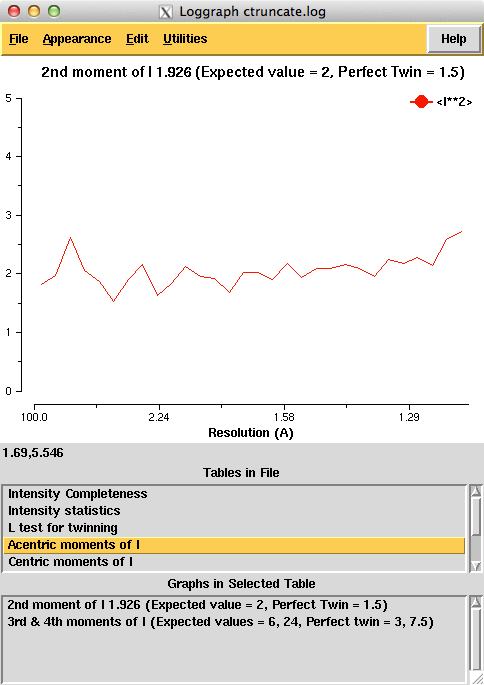
\includegraphics[scale = 0.5]{figures/E4.png}

\end{document}
